\documentclass[a4paper]{article}
\usepackage[T1]{fontenc}
\usepackage[utf8]{inputenc}
\usepackage{fancyhdr}
\usepackage{vmargin}
\usepackage{multirow}	
\usepackage{amsmath}
\usepackage{amssymb}
\usepackage{comment}
\usepackage{graphics}
\usepackage{color}
\usepackage{framed}
\usepackage{epsfig}
\usepackage{subfigure}

\DeclareMathOperator*{\btie}{\bowtie}

\setlength{\parindent}{0pt}
\setlength{\parskip}{5pt}

\frenchspacing
\pagestyle{fancy}
\sloppy 

\markright{headline}


% Macro for grading instructions.
\newcommand{\points}[1]{\qquad\textbf{#1}}

% this should fix the problem with the accented characters in the solutionbox environment
% it is most probably due to the non-UTF8 encoding of the comment.cut file
\renewcommand\ThisComment[1]{%
  \immediate\write\CommentStream{\unexpanded{#1}}%
}

% Definitions for the solution boxes:
%
\includecomment{solution}
\includecomment{notinsolution}

\newenvironment{fshaded}{
  \definecolor{shadecolor}{rgb}{1,.95,.85}
  \definecolor{framecolor}{rgb}{0.6,0.6,0.6}
\def\FrameCommand{\fcolorbox{framecolor}{shadecolor}}
\MakeFramed {\FrameRestore}}
{\endMakeFramed}

\begin{solution}
\specialcomment{solutionbox}
  {\begin{fshaded} {\large \textbf{Loesung:}} }
  {\end{fshaded}}
\end{solution}

\begin{notinsolution}
\specialcomment{notinsolutionbox} {} {}
\end{notinsolution}

% By default we include the solutions.
% Command used for excluding the solutions.
\newcommand{\withoutsolutions}{\excludecomment{solutionbox}
\renewcommand{\nosolutionspagebreak}{\pagebreak}
\renewcommand{\solutionspagebreak}{}}

\newcommand{\nosolutionspagebreak}{}
\newcommand{\solutionspagebreak}{\pagebreak}
\newcommand{\equaltext}[1]{\ensuremath{\stackrel{\text{#1}}{=}}}
\usepackage{ marvosym }

\begin{document}

% Add the title of the assignment sheet and the name of the TA here:
\newcommand{\subtitle}{\textbf{\"Ubungsblatt 2}}
%\newcommand{\TAName}{Endre Palatinus}
\lhead{\begin{tabular}{l}
Informationssysteme SoSe 2017 \\ Information Systems Group \\Saarland University
\end{tabular}}

\rhead{\begin{tabular}{rc} Prof. Dr. Wolfgang Paul &
\multirow{3}{*}{
\includegraphics[scale=0.4]{./CS-UdS-logo.jpg}} \\
	\subtitle  \\
	\ 
 \end{tabular}}
 
 \author{Prof. Jens Dittrich et al.}


% Use this command to exclude solutions. Without that, the solutions are included.
%\withoutsolutions


%%%%%%%%%%%%%%%%%%%%%%%%%%%%%%%%%%%%%%%%%%%%%%%%

\section{ER-Modellierung}

Erstellen Sie ein ER-Modell entsprechend der folgenden Spezifikation. W\"ahlen Sie dabei sinnvolle Schl\"ussel. Markieren Sie au{\ss}erdem schwache Entit\"atstypen und geben sie die Funktionalit\"at in Min/Max-Notation an.

\begin{itemize}
\item Jeder Besucher hat einen Namen und Geld.
\item Besucher besichtigen die Tierh\"auser mit bestimmten Themen, und beobachten Tiere in den Gehegen. Ein Tierhaus kann bis zu 5 Gehege beinhalten, wie zum Beispiel ein Afrika Haus mit Giraffen und Zebras. 
\item Jedes Tier wohnt in genau einem Gehegen mit bestimmter Gr\"o{\ss}e und haben einen Namen.
\item Ein Tier kann h\"ochstens einen Besucher als Paten haben.
\item Da der Zoo sehr stolz auf das Alter seiner Riesenschildkr\"oten ist, soll f\"ur diese zus\"atzlich das Geburtsdatum gespeichert werden.
\item Besucher k\"onnen Shows zu einer bestimmten Uhrzeit besuchen.
\end{itemize}

\begin{solutionbox}
\newline
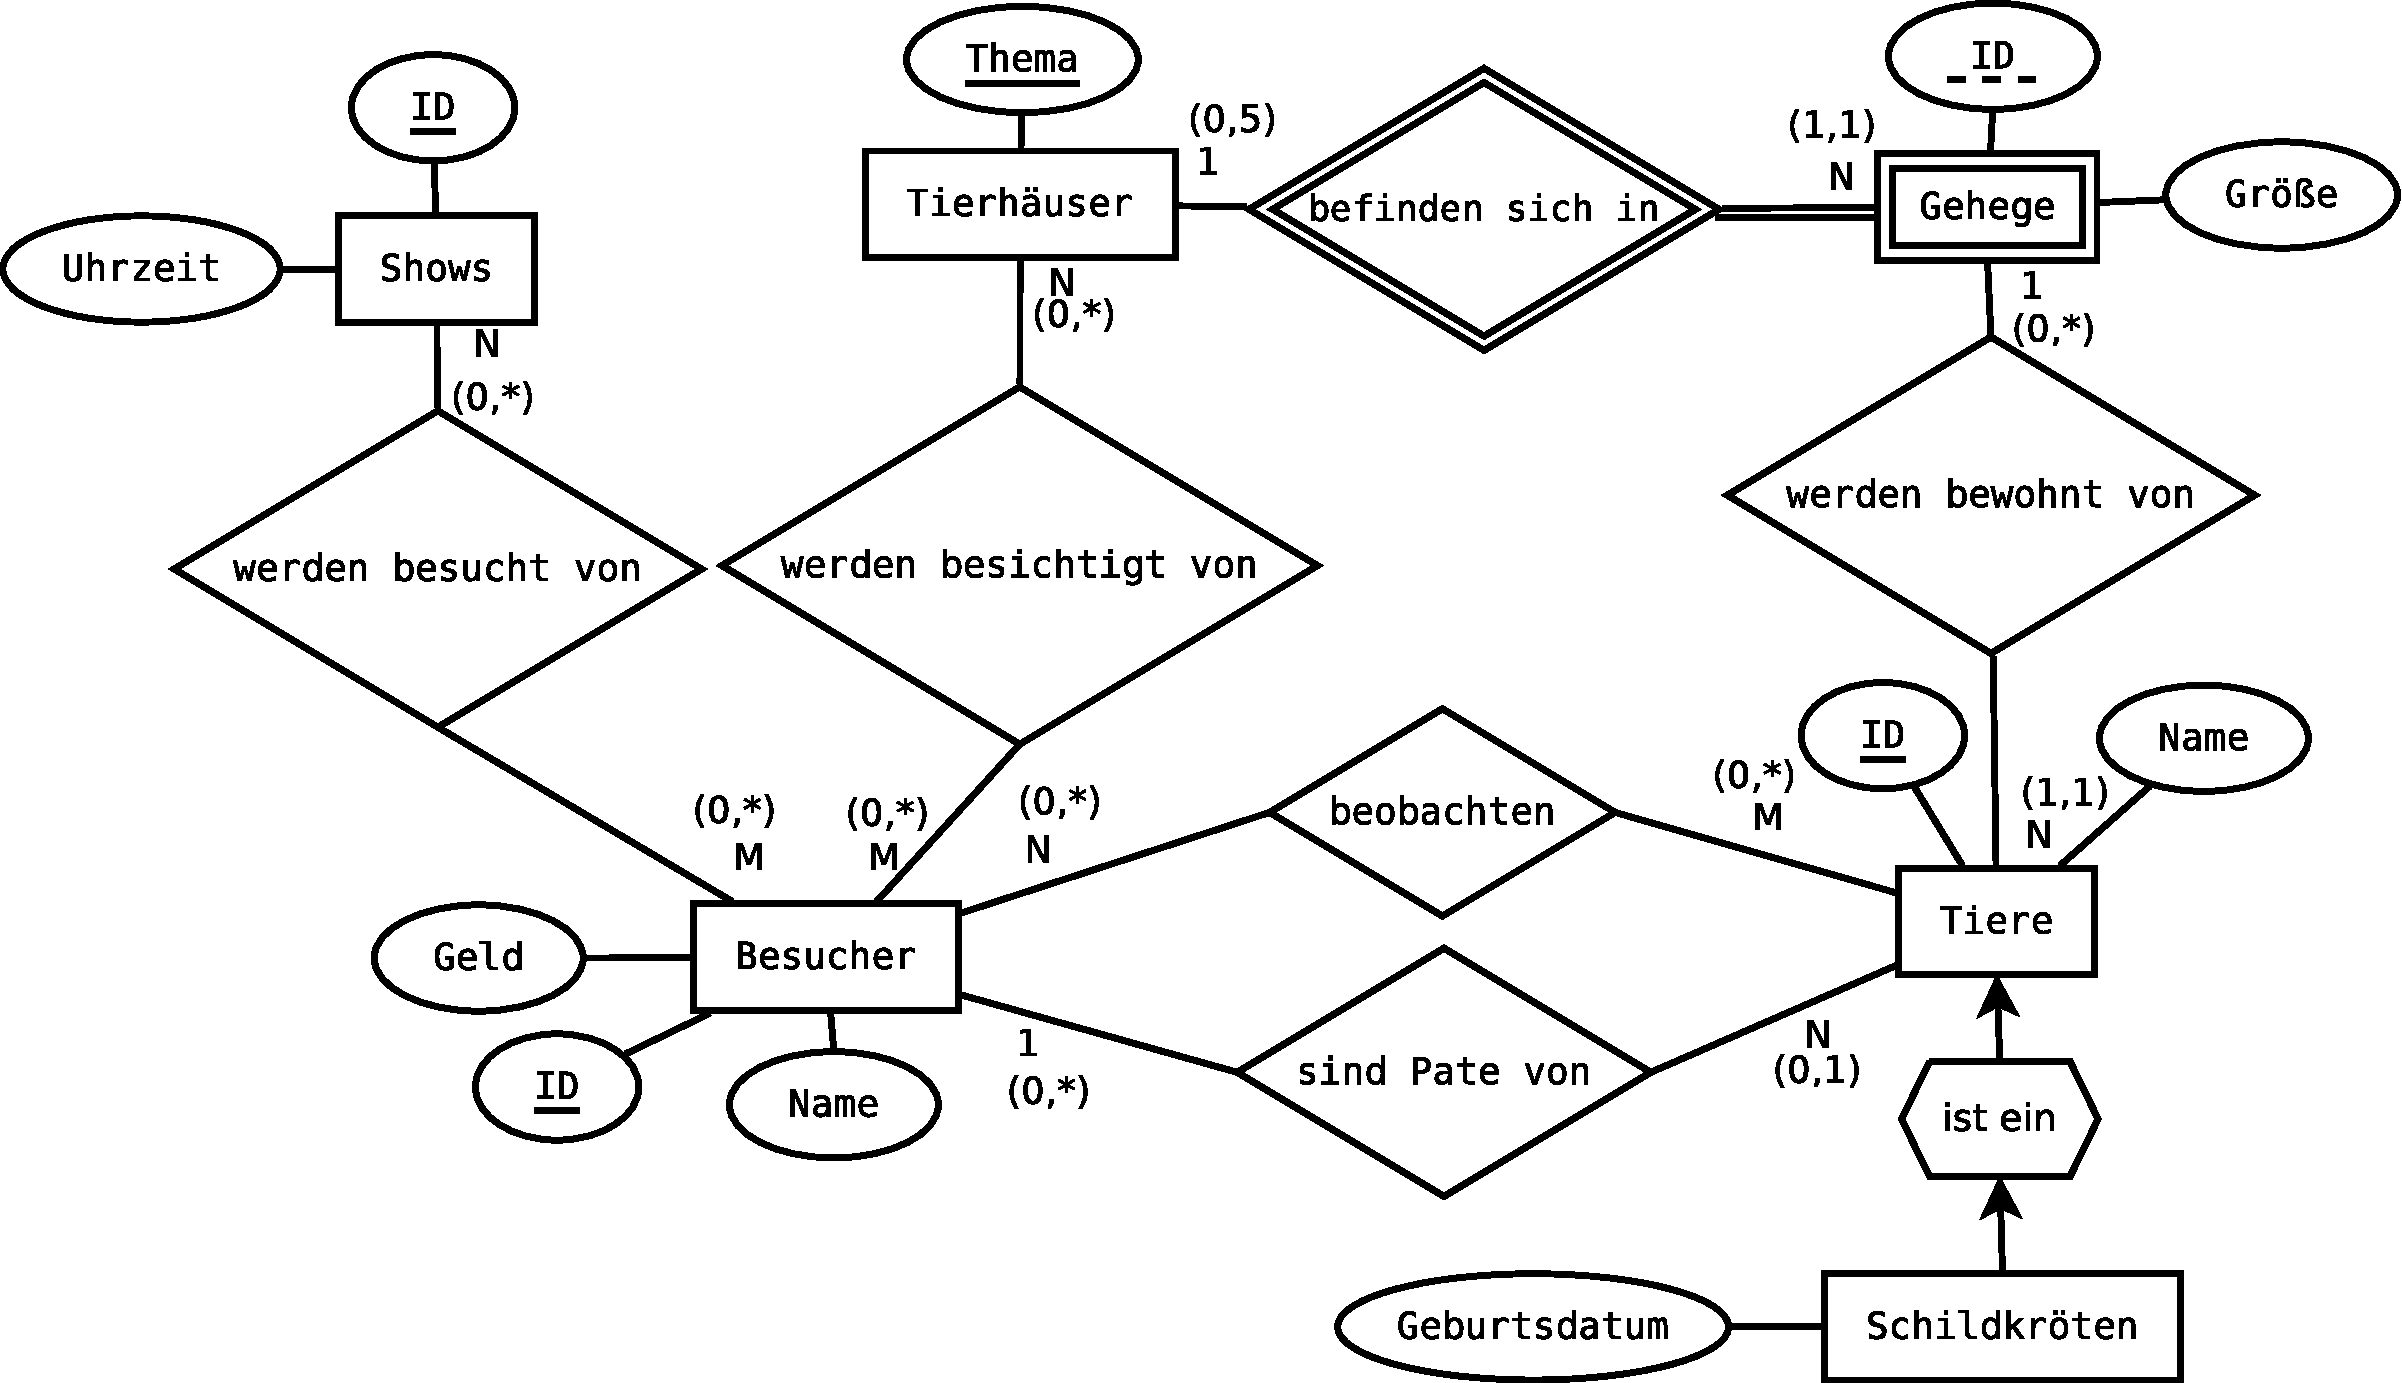
\includegraphics[width=\textwidth]{./a1_ml.pdf}
\end{solutionbox}

%%%%%%%%%%%%%%%%%%%%%%%%%%%%%%%%%%%%%%%%%%%%%%%%

\section{Theorie}

Beweisen Sie Lemma 5, 6, und 7 aus dem Skript.

\begin{solutionbox}
  \newpage
  \subsection{Lemma 5}
  For $A_i \in AB(\mathcal{T})$:\\
  For $x=r$:
  \[
    flat(v).(A_i.A_{i,j}) \equaltext{(1)} v(A_i)(A_{i,j}) \equaltext{(2)} v.A_i.A_{i,j}
  \]
  (1) Definition of flat(.) \\ (2) See page 40 for usage of projection for subcolumns \\

  For $x=t$:
  \begin{equation*}
    flat(v).(A_i.A_{i,j}) \equaltext{(1)} \underbrace{(v_1 \circ \ldots \circ v_n)}_{=vf}.(A_i.A_{i,j})  \equaltext{(2)} vf_{\in\{k:A_k = A_i.A_{i,j}\}} = v.A_i.A_{i,j}
  \end{equation*}
  (1) Definition of flat(.) \\ (2) See page 23 \\ Basically what happens: 
  \begin{align*}
    A_1 & = (A_{1,1},\ldots,A_{1,n}) \\
    A_2 & = (A_{2,1},\ldots,A_{2,n}) \\
    v & = (A_1,A_2) = (\underbrace{(A_{1,1},\ldots,A_{1,n})}_{v_1},\underbrace{(A_{2,1},\ldots,A_{2,n})}_{v_2}) \\
    \longrightarrow \text{flatten and rename} \\
    flat(v) & = (v_1 \circ v_2) = (A_1.A_{1,1},\ldots,A_1.A_{1,n},A_2.A_{2,1},\ldots,A_2.A_{2,n})
  \end{align*}
  
  For $A_i \in AE(\mathcal{T})$ it follows directly from the definition of flat.
  \subsection{Lemma 6}
  For $A_i \in AB(\mathcal{T})$:\\
  For $x=r$:
  \[
    flat(v).A(\mathcal{R}_i) \equaltext{(1)} flat(v)|_{A(\mathcal{R}_i)} \equaltext{(2)} v.A_i
  \]
  (1) See page 23 \\ (2) If flat(v) is restricted to $A(\mathcal{R}_i)$ it is logical that this is $=v.A_i$

  For $x=t$:\\
  Analogue to page 23
  \begin{align*}
    K & = A(\mathcal{R}_i) \equaltext{(1)} \left\{ A_i.A_{i,1},\ldots,A_i.A_{i,n} \right\} \\
    \longrightarrow  \\
    flat(v).K & = flat(v).A(\mathcal{R}_i) = (A_i.A_{i,1},\ldots,A_i.A_{i,n}) \equaltext{(2)} v.A_i
  \end{align*}
  (1) See page 47f After renaming $A(\mathcal{R}_i)$ should be of the form $A_i.A_{i,j}$\\
  (2) Except for renaming

  For $A_i \in AE(\mathcal{T})$ it follows directly from the definition of flat.

  \subsection{Lemma 7}
  Proof by contradiction: \\
  Let $is-key(K,va(t))$ be true and assume $is-key(K',va(flat(t)))$ does not hold. Then
  \begin{align*}
    (1) & \left(\exists v \in va(flat(t)),k' \in K' : v.k' = \bot\right) \vee \\
    (2) & \left( \exists v,v' \in R : v =_{K'} v' \wedge v \neq v' \right)
  \end{align*}
  If (1) holds: \\
  For $k' = A_i.k$:
  \[
    \exists v' \in r_i : v'.k = \bot \wedge k \in K \text{\Lightning}
  \]
  For $k' \in KE$ then by construction $k' \in K$ so $k'$ can not be $\bot$\Lightning

  If (2) holds: \\
  w.l.o.g. \[
    \exists k' \in A(flat(t)), \exists v,v' \in va(flat(t)): v.k' \neq v'.k' \wedge v =_{K'} v' \wedge k' \notin K'  
  \]
For $k' = A_i.k$: Let $K_i$ denote the key of $A_i$. $k \in A(r_i) \wedge k \notin K_i$ must hold, else $k' \in K'$ would be true.\\
But then $K_i$ can not be a valid key for $A_i$ since
\[
  \exists v,v' \in va(A_i) : v =_{K_i} v' \wedge v.k \neq v'.k \text{\Lightning}
\]

For $k' \in AE(t)$:
\[
  \exists v,v' \in va(t) : v =_K v' \wedge v.k \neq v'.k \wedge k \notin K \text{\Lightning}
\]
\end{solutionbox}
\end{document}
